\documentclass[10pt,letterpaper]{article}
% Built by build.py from ../results/*.json. Needs only texlive-latex-base.
\usepackage[T1]{fontenc}
\usepackage[utf8]{inputenc}
\usepackage{lmodern}
\usepackage{textcomp}
\usepackage[margin=1in]{geometry}
\usepackage{amsmath,amssymb}
\usepackage{graphicx}
\usepackage{array,tabularx,longtable}
\usepackage{url}
\usepackage{fancyhdr}
\usepackage{float}

% Characters that appear in data-driven text
\DeclareUnicodeCharacter{2192}{\ensuremath{\rightarrow}}
\DeclareUnicodeCharacter{2190}{\ensuremath{\leftarrow}}
\DeclareUnicodeCharacter{2264}{\ensuremath{\le}}
\DeclareUnicodeCharacter{2265}{\ensuremath{\ge}}
\DeclareUnicodeCharacter{2212}{\ensuremath{-}}
\DeclareUnicodeCharacter{2248}{\ensuremath{\approx}}
\DeclareUnicodeCharacter{0394}{\ensuremath{\Delta}}
\DeclareUnicodeCharacter{2032}{\ensuremath{'}}
\DeclareUnicodeCharacter{220F}{\ensuremath{\prod}}
\DeclareUnicodeCharacter{207B}{\ensuremath{^{-}}}
\DeclareUnicodeCharacter{2070}{\ensuremath{^{0}}}
\DeclareUnicodeCharacter{00B9}{\ensuremath{^{1}}}
\DeclareUnicodeCharacter{2074}{\ensuremath{^{4}}}
\DeclareUnicodeCharacter{2075}{\ensuremath{^{5}}}
\DeclareUnicodeCharacter{2080}{\ensuremath{_{0}}}
\DeclareUnicodeCharacter{1D62}{\ensuremath{_{i}}}
\DeclareUnicodeCharacter{00B2}{\ensuremath{^{2}}}
\DeclareUnicodeCharacter{00B3}{\ensuremath{^{3}}}
\DeclareUnicodeCharacter{2076}{\ensuremath{^{6}}}
\DeclareUnicodeCharacter{2077}{\ensuremath{^{7}}}
\DeclareUnicodeCharacter{2078}{\ensuremath{^{8}}}
\DeclareUnicodeCharacter{2079}{\ensuremath{^{9}}}
\DeclareUnicodeCharacter{2081}{\ensuremath{_{1}}}
\DeclareUnicodeCharacter{2082}{\ensuremath{_{2}}}
\DeclareUnicodeCharacter{2083}{\ensuremath{_{3}}}
\DeclareUnicodeCharacter{2084}{\ensuremath{_{4}}}
\DeclareUnicodeCharacter{2085}{\ensuremath{_{5}}}
\DeclareUnicodeCharacter{2086}{\ensuremath{_{6}}}
\DeclareUnicodeCharacter{2087}{\ensuremath{_{7}}}
\DeclareUnicodeCharacter{2088}{\ensuremath{_{8}}}
\DeclareUnicodeCharacter{2089}{\ensuremath{_{9}}}

\setlength{\extrarowheight}{0.5pt}
\newcolumntype{L}{>{\raggedright\arraybackslash}X}
\newcolumntype{R}{>{\raggedleft\arraybackslash}X}
\setlength{\parskip}{2pt plus 1pt}
\setlength{\parindent}{0pt}
\setlength{\textfloatsep}{8pt plus 2pt minus 2pt}
\setlength{\floatsep}{8pt plus 2pt minus 2pt}
\setlength{\intextsep}{8pt plus 2pt minus 2pt}
\setlength{\abovecaptionskip}{3pt}
\setlength{\belowcaptionskip}{3pt}
\renewcommand{\topfraction}{0.9}
\renewcommand{\bottomfraction}{0.8}
\renewcommand{\textfraction}{0.07}
\renewcommand{\floatpagefraction}{0.85}
\setcounter{topnumber}{3}
\setcounter{bottomnumber}{2}
\setcounter{totalnumber}{4}
\setlength{\LTpre}{4pt}
\setlength{\LTpost}{4pt}
\AtBeginDocument{\setlength{\LTcapwidth}{\textwidth}}
\makeatletter
% compact section headings
\renewcommand\section{\@startsection{section}{1}{\z@}{-9pt plus -2pt minus -1pt}{3pt}{\normalfont\large\bfseries}}
\renewcommand\subsection{\@startsection{subsection}{2}{\z@}{-6pt plus -2pt minus -1pt}{2pt}{\normalfont\normalsize\bfseries}}
\renewcommand\paragraph{\@startsection{paragraph}{4}{\z@}{4pt plus 1pt}{-0.6em}{\normalfont\normalsize\bfseries}}
\makeatother
\pagestyle{plain}
\newcommand{\tablefont}{\normalsize}
\begin{document}
\begin{center}{\LARGE\bfseries A Safe and Reliable MultiPlanetary Exchange System\par}\vspace{3pt}\end{center}
\begin{center}\textbf{Abstract}\end{center}\vspace{-6pt}\begin{quote}

We present a prefunded design for trading equities and a capped futures contract across the nine settlements of the
MultiPlanetary Exchange System. Each settlement runs one exchange. To trade remotely, a client first transfers assets
to an account at the market's exchange over the backbone. The market executes only against balances already on its
ledger. In-transit value is never spendable, so lost, delayed or duplicate packets can increase latency but cannot
create or destroy money or shares.

We evaluate the design with a discrete-event simulator of the network in the brief. Without packet loss, an Earth
client buys 1,000 Ares shares at Mars and receives them at home after 3.07 hours. With random loss, the median is
3.07 hours, the 99th percentile is 7.70 hours, and all 2,000 simulated runs complete. The 300-hour capped futures
contract settles correctly on both rising and falling price paths, with both payouts spendable at home after
328.17 hours. All nine settlements can access every implemented product. Neptune is slowest: a share purchase
completes within 72 hours with probability 0.47 and within 168 hours with probability 0.97.
\end{quote}

\section{Introduction}
We design and test a financial market system for nine settlements, from Mercury to Neptune. We implement equities,
a capped futures contract, and their clearing and settlement. Section~\ref{sec:scope} describes how other products,
including options and currencies, could extend the same framework. All inter-settlement communication passes through
gateways. Exchange operators may use the more reliable backbone for official coordination; clients use local access
or the lossy direct service. Messages can take minutes to hours, packets can be lost, and solar exclusion can block
paths for weeks. No exchange can therefore assume that it knows another exchange's current state.

The design does not require that knowledge. Each balance has exactly one writer, and an exchange acts only on assets
already recorded in its own ledger. Inter-exchange transfers are credited exactly once. Packet loss, delay and
duplication can therefore slow service but cannot change conservation or allow the same asset to be spent twice.
Unlike a distributed commit protocol~\cite{gl}, an exchange never waits for another exchange to agree before changing
its own ledger.

Section~\ref{sec:arch} describes the architecture, Section~\ref{sec:rules} the operating rules, and
Section~\ref{sec:guar} the guarantees and costs. Section~\ref{sec:risk} reports risks found in testing,
Section~\ref{sec:long} covers long-term operation, and Section~\ref{sec:deploy} discusses deployment effects.
The evidence appendix contains the traces, calculations and simulation results supporting the numerical claims.
Unless stated otherwise, all results use epoch 2026-09-22 00:00 TDB.

\section{Architecture}\label{sec:arch}
\subsection{Institutions}
The system has one exchange at each settlement. Each exchange keeps its customer accounts in its own ledger and is
the sole writer of those balances.

Any exchange may host a market. In our scenarios, the stock markets are colocated with their registries and initial
sellers: Ares Habitat at Mars, Belt Works at Ceres, and Terra Fabrication at Earth. Mars also hosts the capped futures
contract; it is well connected to the inner system (Appendix S3), and Bob, the price source, is local.

\begin{figure}[!htb]\centering
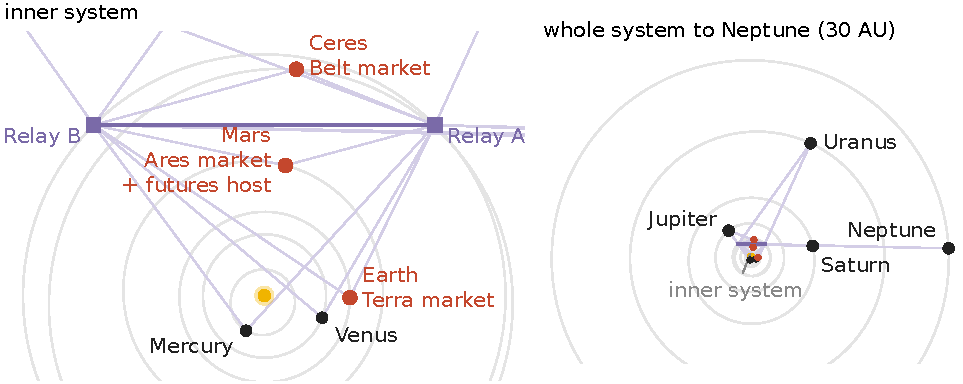
\includegraphics{figs/map.pdf}
\caption{A simplified chart of the nine settlements and two relays. Purple lines represent the 19 backbone links, and red markers are settlements that host a market. Actual flights do not exactly follow straight lines between the positions shown, and a link is closed whenever its path passes within 0.1~AU of the Sun.}\label{fig:map}
\end{figure}

\subsection{Accounts}
Each client has one registered home settlement. A client may also hold a trading account at any of the other eight
exchanges. Remote accounts start empty and receive assets only through explicit transfers via the home exchange. Opening a remote account
does not create money, a new identity or any additional direct-service quota. Table~\ref{tab:owners} summarizes which
institution may change each part of the shared state.

\begin{table}[H]\centering\tablefont\setlength{\tabcolsep}{4pt}
\caption{Ownership of shared state}\label{tab:owners}
\begin{tabularx}{\linewidth}{@{}lL@{}}\noalign{\vskip 1pt}\hline\noalign{\vskip 1pt}\textbf{Shared Information} & \textbf{Governing Institution} \\\hline\noalign{\vskip 1pt}
Available balances, order holds and contract escrow & The exchange that holds those balances \\
Order book and fills & The asset's market exchange \\
Debit and terms of an outgoing transfer & The sending exchange \\
Credit of an incoming transfer & The named receiving exchange, exactly once \\
Share registry (how many shares each exchange holds) & The asset's registry/market exchange \\
Contract positions, fixing and payout allocation & The contract host \\\noalign{\vskip 1pt}\hline
\end{tabularx}
\end{table}

Every run starts from Table~\ref{tab:open}; only clients' home accounts initially hold assets.

\begin{table}[H]\centering\tablefont\setlength{\tabcolsep}{4pt}
\caption{Opening balances}\label{tab:open}
\begin{tabularx}{\linewidth}{@{}lrrrrrrr@{}}\noalign{\vskip 1pt}\hline\noalign{\vskip 1pt}\textbf{Account} & \textbf{Alice} & \textbf{Bob} & \textbf{Cara} & \textbf{Dax} & \textbf{Eve} & \textbf{Fin} & \textbf{Total} \\\hline\noalign{\vskip 1pt}
Home & Earth & Mars & Ceres & Neptune & Uranus & Earth & 5 settlements \\
NeoDollars & \$150,000 & \$50,000 & \$100,000 & \$100,000 & \$50,000 & \$50,000 & \$500,000 \\
Ares & — & 3,000 & — & — & — & — & 3,000 \\
Belt & — & — & 1,000 & — & — & — & 1,000 \\
Terra & — & — & — & — & — & 1,000 & 1,000 \\\noalign{\vskip 1pt}\hline
\end{tabularx}
\end{table}

\subsection{Products and scope}\label{sec:scope}
Table~\ref{tab:scope} lists each product in scope and marks it as implemented or an extension. In either case,
an exchange may act only on assets already in its ledger, and each balance has exactly one writer.

\begin{table}[H]\centering\tablefont\setlength{\tabcolsep}{4pt}
\caption{Status of all products in the brief's scope}\label{tab:scope}
\begin{tabularx}{\linewidth}{@{}p{0.17\linewidth}p{0.13\linewidth}L@{}}\noalign{\vskip 1pt}\hline\noalign{\vskip 1pt}\textbf{Product} & \textbf{Status} & \textbf{Treatment in this framework} \\\hline\noalign{\vskip 1pt}
Equities (Ares, Belt, Terra) & Implemented & They can be bought and sold in units of one share through limit orders at the market exchange (R2), fully prefunded with no end of life. \\
Capped futures & Implemented & Size Q per index point, strike K = 100, collar [60, 140], 300 h term, hosted at Mars, priced by Bob. The long gains when the fixing price P > 100, and the short gains when P < 100. Because P is capped to [60, 140], each side's maximum loss is 40Q, so each side escrows 40Q before opening. The contract ends at fixing with automatic payouts.\\
Clearing and settlement & Implemented & No central counterparty. Delivery versus payment in one ledger write at the host (R2); transfers between exchanges by R1. \\
Capped options & Extension & Writer escrows the maximum payout and the buyer prefunds the premium; settles like R4. \\
Short positions & Extension & The bounded futures short is implemented. Borrowed-share shorts need borrow, return and buy-in rules and are not supported. \\
Bonds and lending & Extension & A loan creates a claim and a liability, not cash. Guaranteed repayment needs escrowed backing; volatile collateral cannot guarantee it. \\
Currencies & Extension & A unit issued by one exchange and fully backed by escrowed NeoDollars, redeemable only there. \\\noalign{\vskip 1pt}\hline
\end{tabularx}
\end{table}

\subsection{Example: an Earth client buys Mars shares}
A cross-settlement trade proceeds in five steps. Figure~\ref{fig:swim} shows these steps for scenario S1a.
\begin{enumerate}\setlength{\itemsep}{1pt}
\item \emph{Funding.} Alice instructs her local exchange, the Earth exchange, to move \$100,000 to her Mars account.
Earth debits her balance immediately and sends a \texttt{TRANSFER} record over the backbone. While the record is in flight, the
money still belongs to Alice, but nobody can spend it.
\item \emph{Import.} Mars accepts the transfer exactly once, credits Alice's Mars account and sends a \texttt{RECEIVED} record
back to Earth.
\item \emph{Order.} When Earth has the receipt, Alice knows that her money is at Mars. She then sends a signed order
to Mars by the direct service. She sends several copies because direct packets are often lost.
\item \emph{Trade.} Mars holds \$100,000 of Alice's cash. It matches her order exactly once against Bob's resting sell order and
exchanges cash for shares in a single atomic step. Bob can spend the proceeds at Mars immediately.
\item \emph{Delivery.} Alice asked for home delivery, so the same atomic step also creates a transfer of her 1,000
shares to Earth. For Alice the trade is complete when Earth credits the shares.
\end{enumerate}

\begin{figure}[H]\centering
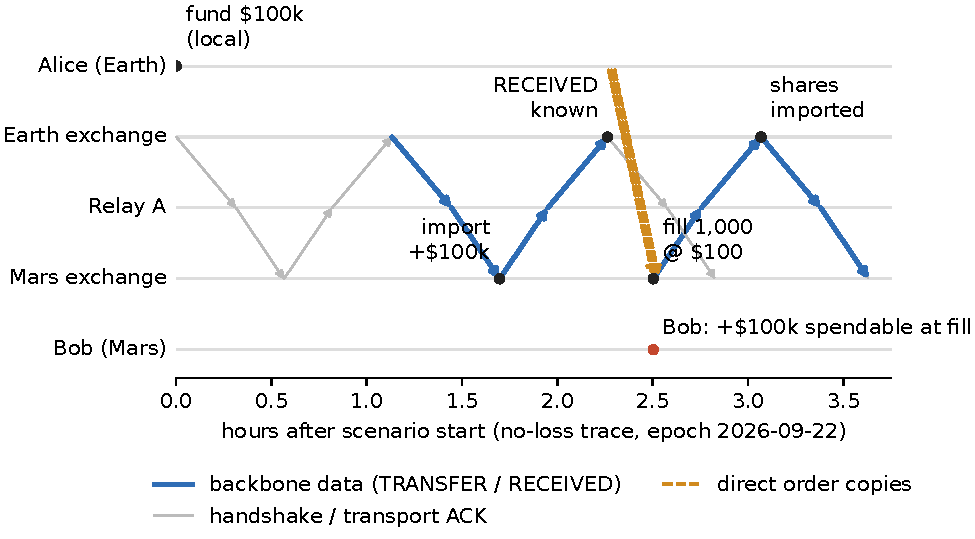
\includegraphics{figs/swimlane_s1a.pdf}
\caption{The S1a trade. Bold arrows carry money or shares. Grey arrows are handshake and acknowledgement packets required by the network. Dashed arrows are Alice's three direct copies of her order. The trade is complete at 3.067 h.}\label{fig:swim}
\end{figure}


\section{Operating rules}\label{sec:rules}
Each rule below states who acts, what information they may rely on and what happens when a message is lost or late.
A change is \emph{durable} if it survives a crash or reset. Every change of financial state described here is a single
atomic, durable write to one exchange's ledger.

\subsection{R1: Moving assets between exchanges}
A TRANSFER record has a globally unique identifier (source exchange and export number), owner, asset, amount,
destination and purpose. Its terms never change.
\begin{enumerate}\setlength{\itemsep}{1pt}
\item The source checks the owner's \emph{available} balance and, in the same atomic write, debits it and creates the
transfer. The value is then ``in transit'' and cannot be spent elsewhere.
\item The destination credits the transfer the first time it sees the identifier and keeps a durable duplicate record
(compacted in Section~\ref{sec:long}). Later copies only cause another \texttt{RECEIVED}.
\item The source marks the transfer delivered when \texttt{RECEIVED} arrives.
\end{enumerate}

A missing \texttt{RECEIVED} never causes a refund: the destination may already have credited the transfer and only the
confirmation may be lost. The network first uses its hop and endpoint retries; if those fail, the source resubmits
the same \texttt{TRANSFER} after 24, 48 and 96 hours and then every 168 hours. Reusing the identifier makes the retries
idempotent. If the destination account is closed, the asset enters a restricted, non-spendable balance and is returned
in a new transfer.

Share transfers always pass through the stock's registry exchange. Shares may move between the registry and a
custodian exchange, but never directly between two custodians. The registry can therefore reconcile how many shares
each exchange holds.

\subsection{R2: Orders, holds and matching}
An order specifies its owner, unique identifier, asset, side, integer quantity, limit price, time-in-force
(good-till-cancelled or immediate-or-cancel), expiry no more than 30 days away, and disposition. The disposition says
whether proceeds stay at the market or are sent home automatically.

The market accepts an order only if the owner's available balance covers it: quantity times limit price for a buy,
or the shares for a sell. Those assets move into a hold that nothing else can use. An uncovered order is rejected
permanently; after funding, the client must submit a new order with a new identifier.

Orders match by price-time priority at the resting order's price, and self-trades are skipped. Each fill is atomic:
the buyer's cash hold and seller's share hold are reduced, the seller receives the trade price, and the buyer receives
the shares plus any price improvement. If the buyer requested home delivery, the same write creates the transfer home.
This is delivery versus payment within one ledger~\cite{pfmi}. An unmatched GTC order rests until filled, cancelled
or expired; an IOC order immediately releases any unfilled remainder. A cancellation releases only the unfilled
portion. If a cancellation arrives before its order, the market records it and rejects the later order. Orders cannot
be amended; they must be cancelled and replaced.

\emph{Listings and quotes.} Ares trades only at Mars, Belt only at Ceres and Terra only at Earth, in whole shares at
whole-NeoDollar prices. Every exchange holds this listing table, so a client can learn locally whether a stock exists
and where it trades before funding. Listing changes are official records sent over the backbone with a future
effective time; none occurs in our scenarios. Each market keeps the authoritative book for its stock. Quotes from R5
are informational snapshots and may be stale. A client therefore submits a limit price rather than relying on a quote
for execution, and the system has no market orders.

Accepted orders have states \texttt{RESTING}, \texttt{PARTIALLY-FILLED}, \texttt{FILLED}, \texttt{CANCELLED} or \texttt{EXPIRED}; rejected orders have state
\texttt{REJECTED}. A remote client learns material state changes through the R5 status mechanism. These reports are
informational only: losing or delaying a report cannot change the order or its financial effect.

\subsection{R3: Withdrawals and account closure}
A \texttt{WITHDRAW} instruction names an amount or \texttt{ALL}; \texttt{ALL} is evaluated once when the host first processes it, and duplicates
return the same transfer. Withdrawals use only available balance and do not cancel orders or touch margin. A \texttt{CLOSE}
instruction rejects new orders, cancels open ones and withdraws the free balance. Escrow remains at the host until
the contract settles, after which payouts are sent home automatically. Only the exchange holding an asset can send
it back.

\subsection{R4: Implemented capped futures and margin rule}
We implement one capped cash-settled futures contract as the tested price-dependent product. Other derivatives may
use different payoff functions, but any supported contract must have a finite maximum loss for each side and fully
escrow that amount before opening.

For the implemented contract, the long and short agree on a size $Q$ in NeoDollars per index point, strike $K=100$,
and collar $[60,140]$. The long's payoff is
\[
Q \times \bigl(\min(\max(P,60),140)-100\bigr),
\]
where $P$ is the fixing price; the short receives the negative.

\emph{Margin rule.} Each side escrows its maximum possible loss before the contract opens. Here that amount is $40Q$
per side, held at Mars until fixing. There is no variation margin, margin call, netting or share collateral. Because
escrow covers the maximum obligation, no price path can create an unfunded liability.

Each party first funds its Mars account (R1) and then sends a contract instruction containing the full terms. Mars
moves that party's margin from available cash into a hold. When both holds exist, the contract opens atomically and
matures 300 hours later. If both margins are not held by the opening deadline, 168 hours after the scenario starts,
the contract is rejected and each hold returns to available balance. A client that has not received \texttt{OPEN} may withdraw
its available balance. At fixing, payout transfers home are created in the same atomic write.

Bob is the named index source at Mars. He publishes one signed observation locally at 60, 120, 180, 240 and 300 hours
after opening. Mars fixes the contract 24 hours after maturity using observation 5. If it is missing, or conflicting
copies exist, Mars uses the latest earlier valid observation, or 100 if none exists. Observations arriving after fixing
are ignored. 

\subsection{R5: Communication services}
Table~\ref{tab:service} assigns each message type to a communication service. The nine exchanges receive 66 of the
600 daily backbone originations each, using 594 in total and avoiding a shared counter. SYN packets, first
transmissions, \texttt{RECEIVED} records and application resubmissions count against this quota; automatic retries and ACKs do
not, although packet totals include every launch. Client instructions do not use the backbone, and exchanges do not
use the direct service for official coordination.

\emph{Quota classes.} A data packet carrying any record other than \texttt{RECEIVED} is \emph{routine} and may be originated
only while the exchange has used fewer than 44 originations in the previous 24 hours. SYN packets, receipt-only
packets and application resubmissions may use all 66, leaving at least 22 originations per exchange for recovery.

\emph{Packet sizes.} Every application record has an 88-byte common header containing type, length, identifier,
creation time and issuer signature. \texttt{TRANSFER} is 176 bytes, \texttt{RECEIVED} 120 bytes, a quote request 120 bytes, a market
snapshot 152 bytes, and a client instruction 128--256 bytes. A network packet has the brief's 64-byte header and at
most 960 payload bytes; our 16-byte sub-header leaves 944 bytes for whole records. Records are never split, and a
packet closes when the next record would not fit.

\emph{Status reports.} Remote clients learn material order and contract state through their home exchange. A market
or contract host batches \texttt{STATUS} entries by destination home exchange and sends them over the backbone; the home
exchange reports them to its client by local access. Equity states are \texttt{REJECTED}, \texttt{RESTING}, \texttt{PARTIALLY-FILLED}, \texttt{FILLED},
\texttt{CANCELLED} and \texttt{EXPIRED}; contract states include \texttt{HELD}, \texttt{OPEN} and \texttt{REJECTED}. Status is informational only and does not
change the underlying financial state. Backbone delivery makes it usable even when the client's direct path is
blocked. Contract-status traffic is already included in Appendix S1 packet counts; an equity status that can share a
packet with an existing transfer or receipt adds no launch, while a standalone status consumes routine backbone
capacity.

\emph{Market data.} Each market can return a 152-byte snapshot containing best bid and ask with sizes, last trade,
book version and timestamp. Every exchange keeps the newest snapshot it has received for each stock on a local
\emph{board}; at the market itself, the board reflects the live book. A client reads its local board and may issue a
\texttt{QUOTE} request to its own exchange. If the snapshot is older than the client's requested freshness, that exchange may
request a new snapshot from the market over the backbone, at most once per stock every 6 hours and shared across its
clients. The request and reply are routine records.

Quotes are not execution guarantees. They may be stale by the time an order reaches the market, so the client's limit
price determines the worst acceptable execution price. Market data is request-driven and never uses the direct
service. In S1a, the quote request fit in Alice's funding packet and the reply fit with \texttt{RECEIVED}, so the scenario's
packet count did not change. 

\begin{table}[H]\centering\tablefont\setlength{\tabcolsep}{4pt}
\caption{Communication service for each message type.}\label{tab:service}
\begin{tabularx}{\linewidth}{@{}LLL@{}}\noalign{\vskip 1pt}\hline\noalign{\vskip 1pt}
\textbf{Message} & \textbf{Service} & \textbf{Quota charged} \\\hline\noalign{\vskip 1pt}
\texttt{TRANSFER} and \texttt{RECEIVED} &
Backbone, fixed route of at most 3 links &
Sending exchange; up to 66 originations per rolling 24 h \\
Order, cancel, withdrawal, close, contract instruction &
Local access at host; otherwise direct &
Client's 12 direct packets per rolling 24 h, at least 60 s apart \\
Price observation &
Local access at Mars (Bob is local) &
None \\
Listing table, local market-data board and \texttt{QUOTE} instruction &
Local access at client's exchange &
None \\
Quote request and snapshot reply &
Backbone between client's exchange and market; at most one request per stock per 6 h &
Request counts against requesting exchange's routine quota; reply against market's routine quota \\
\texttt{STATUS} &
Backbone from host to client's home exchange, then local access &
Host exchange's routine backbone quota; batched by home exchange \\\noalign{\vskip 1pt}\hline
\end{tabularx}
\end{table}

\subsection{R6: Reference client behavior}
Clients are not trusted to enforce financial safety; exchanges enforce balances, holds, identifiers, deadlines and
duplicate handling. Our evidence uses a reference client that knows the published ephemeris but not hidden incidents.
Its behavior affects latency and packet use, but not asset safety.

\begin{itemize}\setlength{\itemsep}{1pt}
\item \emph{Fund first, then instruct.}
The client waits until its home exchange records \texttt{RECEIVED} for the funding transfer before sending the order
or contract instruction, avoiding rejection for insufficient funds.

\item \emph{Read available market data.}
When preparing a remote stock order, the client reads the listing table and local market-data board. It may request
a fresher quote while funding. A stale or missing quote does not block submission; the client chooses its own limit
price, which bounds the execution price.

\item \emph{Direct delivery.}
The client sends the fewest direct copies, 60 seconds apart, needed for at least 99\% delivery probability, up to
8 copies. If the direct path is closed, it uses R8 forwarding through the third settlement with the earliest arrival.

\item \emph{Fallback.}
If no result arrives within twice the round trip plus 6 h (12 h at most for contract instructions), the client
resends the same instruction, directly or through R8, within its 12-per-day quota, until the order expiry,
opening deadline or 30 days. Released cash stays available at the host for withdrawal. The host processes each identifier at
most once, so duplicates have no additional financial effect.
\end{itemize}

\subsection{R7: Recovery}
Ledgers, outboxes and identifier records are durable. After a reset, session expiry or failed network delivery, the
courier opens a new session and resubmits the same records after 24, 48 and 96 hours and then every 168 hours. It
waits out known closures and quota limits and prioritizes recovery traffic. Table~\ref{tab:fail} summarizes failure
handling.

\begin{table}[H]\centering\tablefont\setlength{\tabcolsep}{4pt}
\caption{Failure handling.}\label{tab:fail}
\begin{tabularx}{\linewidth}{@{}p{0.15\linewidth}LLL@{}}\noalign{\vskip 1pt}\hline\noalign{\vskip 1pt}
\textbf{Event} & \textbf{Sender} & \textbf{Receiver} & \textbf{Financial effect} \\\hline\noalign{\vskip 1pt}
\texttt{TRANSFER} lost or late & Has no \texttt{RECEIVED} and resends the same transfer & Knows nothing; value is not spendable there & Value remains in transit and owned by the client \\
\texttt{RECEIVED} lost & Resends \texttt{TRANSFER} & Ignores duplicate and resends \texttt{RECEIVED} & None; value is already spendable at destination \\
Duplicate transfer/order/instruction & --- & Returns original result; changed terms are rejected & None \\
All order copies lost & Resends same order ID after fallback timeout & No order exists & Cash remains available at host \\
Cancel lost or late & Assumes nothing until order state is known & Order may still fill & Fill stands; cancel releases only unfilled quantity \\
Quote stale or lost & May request a fresher quote & Keeps newest snapshot by version & None; limit price bounds execution \\
\texttt{STATUS} lost & Courier resends it & Client may resend original instruction & None \\
Conflicting price copies & --- & Uses latest earlier valid observation & Fixing is final and never revised \\
Host isolated for 72 h & Remote instructions delayed or forwarded & Local matching and maturity continue & Funded payouts wait in durable outbox \\
Exchange reset & Open sessions are lost & Ledger and outbox remain durable & None \\
Forwarder slow or silent & Client retries after fallback timeout & Host sees nothing or a duplicate & None; funds remain at host \\\noalign{\vskip 1pt}\hline
\end{tabularx}
\end{table}

\subsection{R8: Forwarding through a third exchange}
Solar exclusion can block a client's direct path to the host for weeks while the backbone remains connected. Because
client instructions cannot use the backbone, R8 permits forwarding through a third settlement. When the direct path
is closed, the client chooses a settlement whose two direct legs are open and whose route gives the earliest arrival.
\begin{enumerate}\setlength{\itemsep}{1pt}
\item The client wraps its signed instruction in a \texttt{FWD} record with attempt number $k=1,2,\ldots$ and sends it to the
third exchange by direct service, using the R6 copy rule for that leg.
\item The third exchange forwards each new pair (instruction identifier, $k$) once under its own 12-packet rolling
24-hour direct quota, again using the R6 copy rule. Duplicate copies of the same attempt are ignored. The pair is
retained until the instruction expires or its opening deadline passes.
\item The host treats the forwarded instruction exactly like a direct one. It verifies the client's signature, balance
and identifier, so direct and forwarded copies of the same instruction are duplicates.
\end{enumerate}

The forwarding exchange gains no authority: it cannot alter the signed instruction, no asset passes through it, and
it has no financial obligation. The client learns the result through its home exchange using the R5 status mechanism.
If no status arrives before the R6 fallback timer, the client sends attempt $k+1$ through the best route then
available, or directly once the path reopens. Forwarding uses two direct legs and therefore roughly twice as many
direct packets. During the 2028 Mars conjunction, Earth cannot reach Mars directly for 53 days; with R8, S1a
completes in 4.55 hours (Appendix E5).

\section{Guarantees and costs}\label{sec:guar}
We distinguish between properties that the \emph{rules} guarantee in every possible run and properties that the
\emph{model} (orbits, loss law and quotas) makes likely. The first kind holds for any pattern of packet loss, delay or
reordering. The second kind is supported by simulation evidence but is not proven. Table~\ref{tab:guar} lists both.

\begin{table}[H]\centering\tablefont\setlength{\tabcolsep}{4pt}
\caption{Guarantees of the design and the conditions they depend on.}\label{tab:guar}
\begin{tabularx}{\linewidth}{@{}lp{0.3\linewidth}LL@{}}\noalign{\vskip 1pt}\hline\noalign{\vskip 1pt}\textbf{} & \textbf{Guarantee} & \textbf{Reason} & \textbf{Condition} \\\hline\noalign{\vskip 1pt}
G1 & The total of NeoDollars and of each share type never changes & Every write debits and credits equal amounts; value in transit is a ledger state & Rules only; checked after every event of every traced run \\
G2 & No asset is used for two purposes at once & Available, held, escrowed and in-transit balances are separate & Rules only \\
G3 & Every futures payout is fully funded & Escrow equals the maximum loss and is posted before opening & Rules only; holds for any price path \\
G4 & Each transfer is credited exactly once & The destination keeps a durable record of every credited identifier & Rules and durable storage \\
G5 & A fill is final and immediately spendable at the host & Both holds exist before the atomic fill & Rules only \\
G6 & A funded transfer eventually arrives & Retries never stop, the backbone is always connected, and admission keeps work within quota & Model; under random loss there is no fixed deadline \\
G7 & Completion times & Measured in simulation & Model; see Table~\ref{tab:access} \\\noalign{\vskip 1pt}\hline
\end{tabularx}
\end{table}

\subsection{Service at every settlement}
Every implemented product is accessible from every settlement. Clients can fund and withdraw at all three stock
markets, trade Ares, Belt and Terra shares, and enter the capped futures at Mars. Only latency and completion
probability vary by settlement; Table~\ref{tab:access} summarizes both. \textit{Backbone min} is the one-way delay in minutes to the Mars, Ceres and Earth hosts. \textit{Copies, P} represent the direct copies per instruction to Mars and the probability that at least one arrives. The next three columns are for a \$100,000 Ares purchase with home delivery: completion time in hours without loss, the median under random loss, and the probability of completing within 72 hours (1,000 runs each; Appendix S3).

\begin{table}[H]\centering\tablefont\setlength{\tabcolsep}{4pt}
\caption{Service at each settlement at hour 0.}\label{tab:access}
\begin{tabularx}{\linewidth}{@{}lllrrrL@{}}\noalign{\vskip 1pt}\hline\noalign{\vskip 1pt}\textbf{From} & \textbf{Backbone min} & \textbf{Copies, P} & \textbf{No loss} & \textbf{Median} & \textbf{P(72 h)} & \textbf{Notes} \\\hline\noalign{\vskip 1pt}
Mercury & 42 / 42 / 46 & 3, 0.997 & 3.8 & 3.8 & 1.00 & Direct path to Mars closed from h 22 to h 357; instructions are forwarded (R8) \\
Venus & 37 / 36 / 41 & 3, 0.997 & 3.3 & 3.3 & 1.00 & Closed near Venus–Mars conjunctions; instructions are forwarded (R8) \\
Earth & 34 / 33 / local & 3, 0.998 & 3.1 & 3.1 & 1.00 & Terra local. Direct path to Mars closed about 53 days every 2.1 years; forwarded (R8) \\
Mars & local / 30 / 34 & local & 0.0 & 0.0 & 1.00 & Ares and futures local; Belt (Ceres) and Terra (Earth) remote \\
Ceres & 30 / local / 33 & 2, 0.992 & 2.6 & 2.6 & 1.00 & Belt local; Ares and futures (Mars) and Terra (Earth) remote \\
Jupiter & 40 / 41 / 51 & 4, 0.992 & 3.9 & 4.0 & 1.00 & 4 copies per instruction \\
Saturn & 76 / 75 / 79 & 7, 0.990 & 7.6 & 10.6 & 1.00 & 7 copies per instruction \\
Uranus & 155 / 154 / 158 & 8, 0.885 & 15.4 & 26.8 & 0.99 & 8 copies; the fallback is often used \\
Neptune & 247 / 246 / 250 & 8, 0.545 & 24.7 & 74.4 & 0.47 & 8 copies still all fail 46\% of the time \\\noalign{\vskip 1pt}\hline
\end{tabularx}
\end{table}

Table~\ref{tab:access} uses the Ares purchase; Appendix S3 repeats the test for every implemented product and
settlement. A market is local only at its host: Ares and futures at Mars, Belt at Ceres, and Terra at Earth. For
remote share purchases, the three products finish within 1.1 hours of one another without loss because client
location dominates the delay.

Every futures party must reach Mars before the 168-hour opening deadline. Parties in the inner system almost always
do: in all 2,000 simulated runs with random loss, the contract opened (Appendix E2). For a Neptune party (Dax long against Cara), the contract opened before the deadline in 99.7\% of runs with random loss. In the other runs it was rejected at the deadline and all margin was returned (Appendix S3).

\subsection{Efficiency}

The design's safety guarantees hold in every evaluated scenario: money and shares are conserved, assets cannot be
spent twice, and every accepted obligation is fully funded. The remaining tradeoff is efficiency, mainly in
communication and capital use.

\emph{Communication efficiency} is the total number of direct and backbone packets divided by completed transactions.
A remote equity purchase in S1a uses 15.7 packets per transaction. Reusing an already funded account is cheaper:
S1i completes four fills, a cancellation, a cancel--fill race and a final transfer home at 8.4 packets per
transaction. The capped futures contract uses 28.2 packets per transaction because opening, status reporting,
fixing and payout require more communication.

\emph{Capital efficiency} measures how much NeoDollar value must be encumbered to support the value settled.
S1a has a ratio of 0.33, while the capped futures contract has a ratio of 0.31. The ratio alone does not show how
long capital is unavailable, so we also report asset-hours. In S1d/e, \$160,000 remains encumbered for 324 hours,
or 51.84 million dollar-hours. This prolonged capital lockup is the main economic cost of fully prefunding the
futures contract.

\section{Risks}\label{sec:risk}
Table~\ref{tab:risk} lists weaknesses found through incident search, shifted-epoch runs and outer-settlement tests,
ranked by expected harm under our evidence. The most important arise from interactions between protocol rules and
orbital geometry.

\begin{longtable}{@{}p{0.03\linewidth}p{0.17\linewidth}p{0.36\linewidth}p{0.39\linewidth}@{}}
\caption{Risks found during testing, ranked by harm and likelihood.}
\label{tab:risk}\\
\noalign{\vskip 1pt}\hline\noalign{\vskip 1pt}
\textbf{} & \textbf{Risk} & \textbf{Evidence} & \textbf{Treatment} \\
\hline
\endfirsthead

\multicolumn{4}{l}{\small\itshape Table~\ref{tab:risk} continued from previous page.}\\
\noalign{\vskip 1pt}\hline\noalign{\vskip 1pt}
\textbf{} & \textbf{Risk} & \textbf{Evidence} & \textbf{Treatment} \\
\hline
\endhead

\hline
\multicolumn{4}{r}{\small\itshape Continued on next page.}\\
\endfoot

\hline
\endlastfoot

1 & A solar conjunction cuts a client off from its host
& During the 2028 Mars conjunction the Earth--Mars direct path is closed for 53 days. Earth clients cannot order, cancel or withdraw at Mars. Bob's 30-day sell order expires first, so the trade does not happen (E5).
& Rule R8 forwards instructions through a third exchange (Mercury here): the trade completes in 4.55 h and both futures runs complete. \\

2 & Money left at a host can become unreachable
& Withdrawals are client instructions sent by direct service. Money left at Mars during a closure cannot be called home, even though the backbone still works.
& Clients fund just before they trade (R6). Home delivery and payouts need no instruction. A withdrawal can be forwarded through a third exchange (R8). \\

3 & Direct loss of 76--91\% per copy at the outer settlements
& From Neptune, $P(\text{complete within 72 h}) = 0.47$, because 8 copies only succeed 54\% of the time (S3).
& Up to 8 copies of direct packets are sent, to balance tight quota limits with the high chance of packet loss for outer settlements. \\

4 & Concentration at the host
& All futures margin and the price source are at Mars. An isolation of Mars around the fixing delays both payouts by up to 75 h (S2 search).
& Fixing and payout are local and automatic. Payouts wait, already funded, in the outbox. \\

5 & A direct path can close after funding but before the next instruction
& In an earlier design, Mercury funded Mars shortly before the Mercury--Mars path closed from h 22 to h 357, leaving the client unable to instruct the host directly (S3).
& R8 removes the dependence on a continuously open direct path by forwarding instructions through a third settlement. \\

6 & Sessions are silently lost after an exchange reset
& The worst of 56,280 simulated incidents (S2) is a Mars reset at h 0.75, just after the handshakes. Mars silently drops the funding transfers, and the senders wait about 100 h for endpoint retries plus a 24 h backoff. The futures complete at 453.79 h instead of 328.17 h. The contract still opens before the deadline, and no money is at risk.
& Alternative A1: after a reset, the exchange sends a restart notice to its recent peers. The futures then complete at 329.49 h. A1 is not part of the evaluated design; it is the first change for the next revision. \\

7 & Status reports at scale
& If Mars reported to each remote client by direct service, its 12 direct packets per day would cover at most 12 status changes a day for all clients together.
& Status travels as batched \texttt{STATUS} records to home exchanges over the backbone (R5), at most one entry per client per 6 h unless the state changes. Clients still rely on fallbacks. \\

8 & Single price source
& Bob may fail or publish conflicting copies.
& The fixing falls back to the latest valid earlier observation, or 100. This basis risk is disclosed. \\

9 & Trust in the custodian exchange
& Prefunding concentrates exposure on the host exchange.
& The brief assumes operators follow the rules. Independent audit is future work. \\

\end{longtable}


\section{Long-term operation}\label{sec:long}
\paragraph{The backbone never disconnects.} The two relays are 90\textdegree{} apart on the same circular orbit, and
the link between them always passes at least 2~AU from the Sun. A link between a settlement and a relay is blocked
only when the settlement is almost directly behind the Sun as seen from that relay, at an angle of at least
159\textdegree. This cannot happen for both relays at the same time. Every settlement therefore always has a route of
at most three links to every other settlement, except during maintenance and incidents. Our 200-year scan confirms
this: every settlement had a route to every market host at all 1,753,201 hourly samples. The slowest
one-way route observed was Mars to Neptune at 315 minutes. Because a route has at most three links, its
length is at most $(r_a + R) + 4 + (r_b + R)$~AU at any time, where $r_a$ and $r_b$ are the aphelion distances of the two
settlements and $R = 2.83$~AU is the relay radius. With empty queues this bounds every one-way route delay for all time;
the largest bound is 358 minutes (Neptune to Ceres). Direct paths, in contrast,
do close for weeks at a time during conjunctions, so every promise that depends on the direct service without rerouting is conditional.

\paragraph{Long outages and the backlog afterwards.} Only two things have a deadline: orders, which expire after at
most 30 days and release only their own hold, and contract opening deadlines, which return the margin. Transfers,
receipts and payouts wait in durable outboxes. Sessions that are idle for 7 days are reopened. A packet that reaches
the network's 30-day lifetime is replaced by an application resubmission with the same financial identifier. When a
route reopens, each exchange works through its outbox in packets of five transfers, within its 44 routine
originations per day. We say a backlog has \emph{cleared} when every transfer is credited at its destination and the
source holds every \texttt{RECEIVED}. In simulation (Appendix E6), with no competing traffic, 300 transfers from Earth to Mars
are credited within 24.6 hours and resolved within 25.1 hours of the route reopening, and in at most
30 hours in 20 runs with random loss. Other work from the same
exchange shares the 44 routine originations: 300 transfers to each of the eight peers clear in about
10 days.

\paragraph{Obligations further in the future.} A contract stores its maturity and fixing times as absolute times.
The fixing is a local computation at the host, and the payout transfer is created in the same write. A maturity
several years away therefore needs no message in order to take place.

\paragraph{Capital.} New capital can enter only through fees or contributions debited from real accounts and moved
by R1. Escrow is released only by fixing or rejection; the system creates no free capital.

\paragraph{Storage and identifiers.} An identifier is 12 bytes: a 32-bit principal prefix and a 64-bit counter. At a
million identifiers per second one principal's counter lasts about 585,000 years. Times are stored as signed 64-bit integer milliseconds,
which covers about 292 million years in each direction. Our simulator uses floating-point seconds, which can no longer
resolve 1~ms after 142,710 years, so a production system must use integer time and
extended-precision orbital phase. State is bounded: at most 32 live orders per client per host, 256 per host, and 4,096
export slots per host, each an unresolved transfer or a reservation. A remote client's contract instruction reserves
its payout's slot and a home-delivery order its delivery's (one delivery in transit per order). An instruction is
refused if the slots it needs would take the total past 3,276 (80\%), so every payout and delivery has its slot before
it exists. A late top-up to a closed account waits in a restricted balance, owned by the client, until a slot is
free, so slots in use never exceed 4,096.

\paragraph{Compaction without losing duplicate protection.} A source numbers its transfers to each destination
consecutively and sends them in that order. When a transfer is credited, the destination replaces the full record by a \emph{tombstone}: the
transfer identifier, the final state \texttt{CREDITED} and a 32-byte hash of the terms. A later copy that matches a tombstone
only causes another \texttt{RECEIVED}, and a copy whose terms do not match the hash is rejected. For each source the destination
also keeps a \emph{watermark} $W$, the highest number such that every transfer up to $W$ has been credited. Tombstones
at or below $W$ are dropped, because any identifier at or below $W$ is known to be a duplicate. A source does not send
transfer $n$ while any transfer numbered $n - 512$ or lower is unresolved, so every credited transfer above $W$ lies within
512 of it: at most 512 tombstones per source, however long a gap stays open. The source compacts its own export to a tombstone when the
\texttt{RECEIVED} arrives. Order and instruction identifiers are compacted the same way, and any copy that arrives after the
order's expiry or the contract's opening deadline is rejected on that ground alone. The result of a withdrawal,
funding, cancel or close request is kept for 60 days, and a copy older than 30 days is rejected. Transport packet IDs
follow the brief's own retention rule. A 52-byte closure record diverts late top-ups until the host's watermark passes the home's last
funding sent before it learned of the closure; a contract tombstone lasts until its instructions expire (Supplement E6;
design rules, not simulated). Full records can move to an
off-line audit archive; the live ledger needs only balances, open records, tombstones above the watermarks and one
watermark per peer. When a limit is reached the exchange refuses new work; an obligation it has accepted already
holds the capacity it needs.

\paragraph{Accepted demand.} Each exchange can make up to 44 routine backbone originations per day, which is enough
for about 10 new funding or withdrawal transfers between exchanges at 4 to 5 originations each, plus 22 originations
for recovery. Market data adds one reply per request, at most 4 a day for
each exchange and stock (32 a day at a market), and nothing when no one asks. Each client has 12 direct packets per day, which is enough for 1 to 4 remote instructions depending on
distance. A forwarding exchange (R8) also has 12 direct packets per day, so it can forward 1 to 4 instructions a day. Work beyond this is queued, and we make no promise about its timing.

\paragraph{Very long horizons.} The connectivity argument and the delay bound above depend only on the shapes of the
orbits, so they hold at every time in the model. The scanned statistics (availability, closure counts and typical
delays) describe only the 200 scanned years. The orbital periods are not commensurate, so the joint configuration of
the bodies never repeats exactly, and we do not extend those numbers beyond the scan. Our evidence for later epochs is
the runs at +1, +10 and +100 years (Appendix E5). With integer milliseconds and extended-precision phase, nothing in the rules depends on the date. The remaining limits are the identifier space described above and the physical infrastructure, which the brief
fixes.


\section{Deployment assessment}\label{sec:deploy}
The baseline omits several real effects that would change latency or loss rates but not the ledger rules that enforce
conservation and exclusive use. Table~\ref{tab:deploy} estimates their size.

\begin{table}[H]\centering\tablefont\setlength{\tabcolsep}{4pt}
\caption{Effects a real deployment would add.}\label{tab:deploy}
\begin{tabularx}{\linewidth}{@{}p{0.15\linewidth}p{0.2\linewidth}LL@{}}\noalign{\vskip 1pt}\hline\noalign{\vskip 1pt}\textbf{Effect} & \textbf{Estimated size} & \textbf{Source and assumptions} & \textbf{Effect on the guarantees} \\\hline\noalign{\vskip 1pt}
Earth rotation & About 11.97 h without view per ground station per day & Sidereal day of 23.93 h, one equatorial station, no elevation mask [1] & Delays only, up to 12 h per hop with one station; G1–G5 unchanged. \\
Doppler shift & About 3.20 MHz at 32 GHz & f·v/c with an assumed line-of-sight speed of 30 km/s [1, 2] & Modems track it; otherwise more loss, which only slows service. \\
Relativistic clock rates & Mercury vs Earth: 2.3 × 10⁻⁸, or 0.7 s per year & GM/(rc²) + v²/(2c²) at 0.39 AU and 1 AU & Maturity and fixing use TDB; local clocks are corrected. \\
Ephemeris drift & Not estimated & Kepler elements ignore perturbations between planets & Timetables need a live ephemeris. \\\noalign{\vskip 1pt}\hline
\end{tabularx}
\end{table}

\begingroup\tablefont
\begin{thebibliography}{9}\setlength{\itemsep}{0pt}
\bibitem{fact} NASA, Earth Fact Sheet. \url{https://nssdc.gsfc.nasa.gov/planetary/factsheet/earthfact.html}
\bibitem{esa} ESA, Cebreros DSA-2 ground station (Ka-band, 32 GHz).
\bibitem{pfmi} CPMI--IOSCO, \emph{Principles for Financial Market Infrastructures} (delivery versus payment), 2012.
\bibitem{gl} J.~Gray and L.~Lamport, Consensus on Transaction Commit, \emph{ACM TODS} 31(1), 2006.
\end{thebibliography}
\endgroup

\end{document}